\section{Personal comments}
\label{sec:personal}

My pursue for a PhD degree is now almost one year underway, so this is a good time to reflect how I personally experienced this. When looking back, I realize that there are some areas I can improve upon. Few points for improvements are mentioned in \cref{sec:evaluation}, but first some other personal comments are listed:
\begin{itemize}
	\item I am very satisfied with my choice for Bart De Schutter as a supervisor from the DUT and I am grateful that he accepted to supervise me. I am amazed by the comprehensiveness and accurateness of his comments and his patience to explain his remarks (again and again).
	\item I am also very satisfied with my supervisors from TNO, Jan-Pieter Paardekooper and Olaf Op den Camp. The discussions I have with them are a huge inspiration for me.
	\item Most importantly, I am still enjoying my pursue for a PhD degree every day. I still feel enthusiasm when talking about my PhD and I am very eager to continue every day with my PhD and work at TNO. 
\end{itemize}

\subsection{Self-evaluation}
\label{sec:evaluation}

I am aware that there are many points for improvement. To limit the following list, I selected two points that probably deserve most attention.

\begin{itemize}
	\item \emph{Time management}:
	\item \emph{Stakeholder management}:
\end{itemize}

\begin{figure}[b]
	\centering
	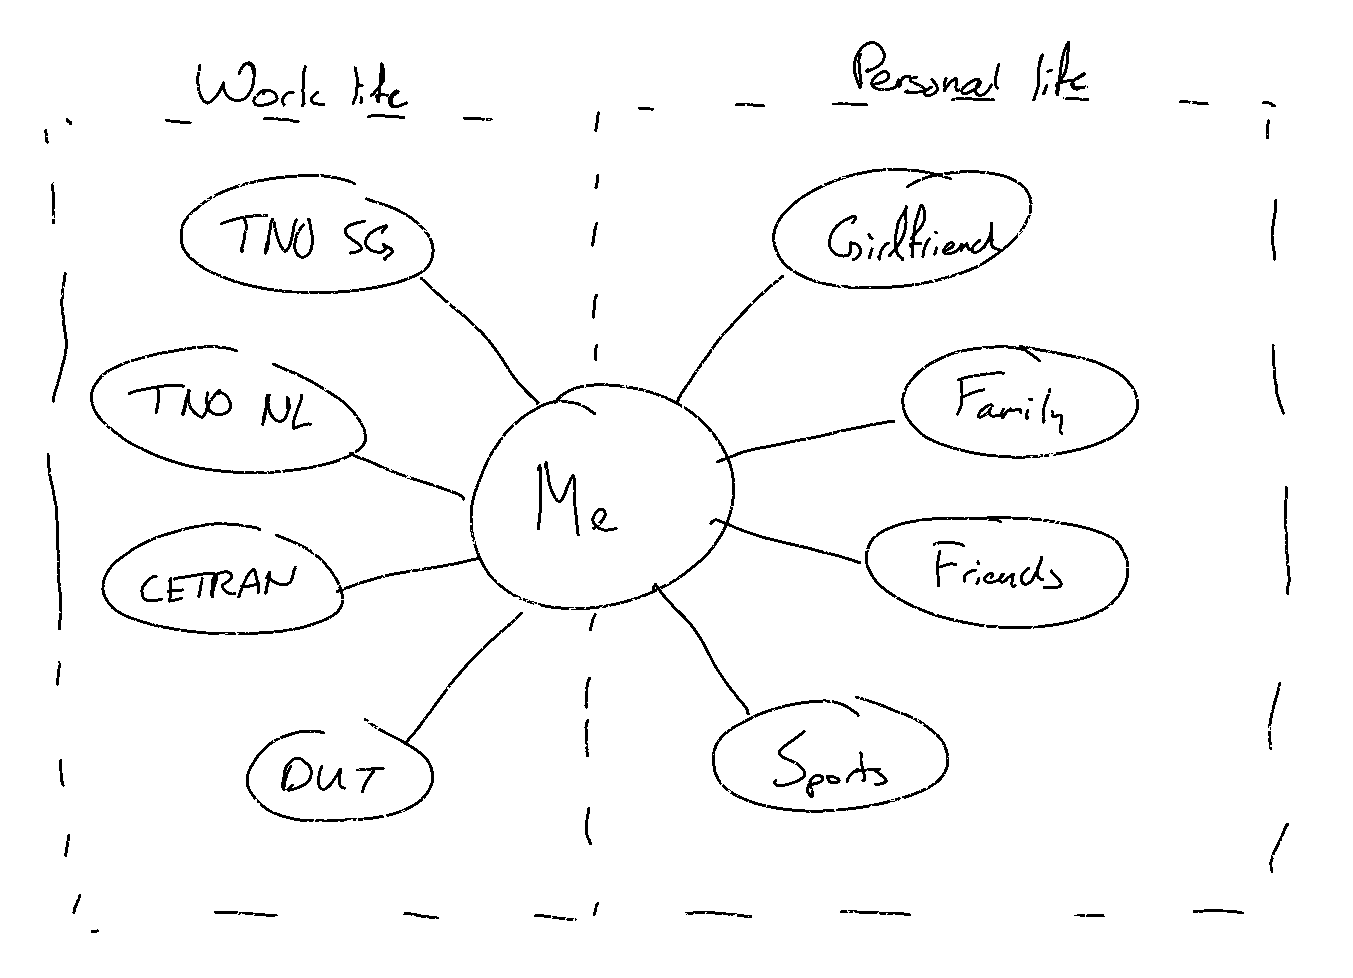
\includegraphics[width=\linewidth]{figures/stakeholders}
	\caption{Overview of the different stakeholders that are involved in either my work or personal life.}
	\label{fig:stakeholders} 
\end{figure}

%\subsection{Graduate school}
%\label{sec:graduate school}
